\section{Materials}

\subsection{Environment}


The vast majority of commands used in this tutorial have been carefully tested and fully executed on a remote linux server working with the Sun Grid Engine (SGE) workload manager. Obviously, Bash scripts presented here will need to be slightly adapted to be used with your own raw sequence data. In addition, other small changes will be required  to these scripts if another workload manager is in place on your computer cluster or if you intend to perform the analysis on a local machine.

\subsection{Installing bioinformatic programs}

\subsubsection{The GATK suite}

It is suggested to install the GATK suite in a separate conda environment. Assuming that you are familiar with the conda package management system, you could install all GATK programs in an environment called 'gatk4' with the following command:

\begin{verbatim}
conda create -n gatk4 -c bioconda gatk4 
\end{verbatim}

To generate optional plots in the Base Quality Score Recalibration subsection, additionnal libraries are required. Use the following commands to install them alongside GATK in the gatk4 environment:

\begin{verbatim}
conda activate gatk4
conda install -c conda-forge r-base
conda install -c r r-ggplot2
conda install -c r r-gplots
conda install -c bioconda r-gsalib
\end{verbatim}


\subsubsection{The NCBI SRA toolkit programs}

You can easily download public sequences from the NCBI Sequence Read Archive (SRA) using the NCBI SRA toolkit. Detailed instructions about this tool can be found at \href{https://trace.ncbi.nlm.nih.gov/Traces/sra/sra.cgi?view=toolkit_doc}{https://trace.ncbi.nlm.nih.gov/Traces/sra/sra.cgi?view=toolkit\_doc}. However, before using it, do not forget to configure the SRA toolkit program ( \href{https://github.com/ncbi/sra-tools/wiki/03.-Quick-Toolkit-Configuration}{https://github.com/ncbi/sra-tools/wiki/03.-Quick-Toolkit-Configuration}).


Once installed, export the SRA toolkit programs in you PATH:

\begin{verbatim}
export PATH=$PATH:$PWD/sratoolkit.2.10.9-ubuntu64/bin
\end{verbatim}

As usual, you can make this change persistent, by adding the previous line to your .bashrc file.


\subsubsection{The STAR aligner}

Although you can retrieve and install the STAR aligner with conda, it can be installed easily by just downloading the latest STAR source from releases:

\begin{verbatim} 
wget https://github.com/alexdobin/STAR/archive/2.7.7a.zip
unzip 2.7.7a.zip
cd STAR-2.7.7a/
\end{verbatim}

You can safely use the pre-compiled STAR executables located in the bin/ subdirectory. It is convenient to add the executables to your PATH:

\begin{verbatim}
export PATH=$PATH:$PWD/bin/Linux_x86_64
\end{verbatim}



\subsubsection{The Picard tools}

We will use the Picard tools (\href{https://broadinstitute.github.io/picard/}{https://broadinstitute.github.io/picard/}) to mark duplicated reads. One can download the pre-build java program with:

\begin{verbatim}
wget https://github.com/broadinstitute/picard/releases/download/\
2.25.0/picard.jar
\end{verbatim}

It is recommend to set up an environment variable to act as a shortcut. Again, to make it persistent in other sessions, simply, add a line to your .bashrc file:

\begin{verbatim}
export PICARD=$HOME/bioinfo_programs/picard.jar
\end{verbatim}

Then, you would be able to call Picard tools with:

\begin{verbatim}
java -jar $PICARD
\end{verbatim}


\subsubsection{Samtools, BCFtools and HTSlib}


The Samtools web site (\href{http://www.htslib.org/}{http://www.htslib.org/}) contains a plenty of informations about the Samtools suite, a collection of widely used bioinformatic programs designed to read, write, edit, index and view alignments files in the SAM, BAM and CRAM formats \cite{Danecek2021}. Less known, but just as powerful, the BCFtools are the best option to manipulate sequence variants stored in the BCF2, VCF and gVCF format. The HTSlib is a C library designed to read and write high-throughput sequencing data that is used by both the Samtools and the BCFtools. It notably contains the tabix and bgzip indexing and compression utilities.

Since the Samtools, the BCFtools and the HTSlib projects are now divided in three separated repositories, the most straightforward way to make use of these three distinct packages is to build them independently. 

Use the commands below to install the Samtools (and similarly for the BCFtools and HTSlib):

\begin{verbatim}
wget https://github.com/samtools/samtools/releases/download/\
1.11/samtools-1.11.tar.bz2
bzip2 -d samtools-1.11.tar.bz2	
tar -xvf samtools-1.11.tar
cd  samtools-1.11
./configure --prefix=$HOME/bioinfo_programs/samtools-1.11
\end{verbatim}

And you may wish to add the bin directory to your \$PATH:

\begin{verbatim}
export PATH=$PATH:$HOME/bioinfo_programs/samtools-1.11/bin
\end{verbatim}

\subsection{Downloading scripts used in this tutorial}

A good starting point would be to download the following GitHub repository:

\begin{verbatim}
git clone https://github.com/soda460/RNAseq_GATK_JGW.git
\end{verbatim}

It contains all scripts described in the next sections as well as several text files that allow one to reproduce the analysis presented here. Consistent with the GitHub repository, figure 2 displays the relative organization of the scripts, files and folders refered by, or created by the listings described in this tutorial. Albeit somes files and subfolders were omited, it gives a good overview of the entire workflow.


\begin{figure}
\begin{center}

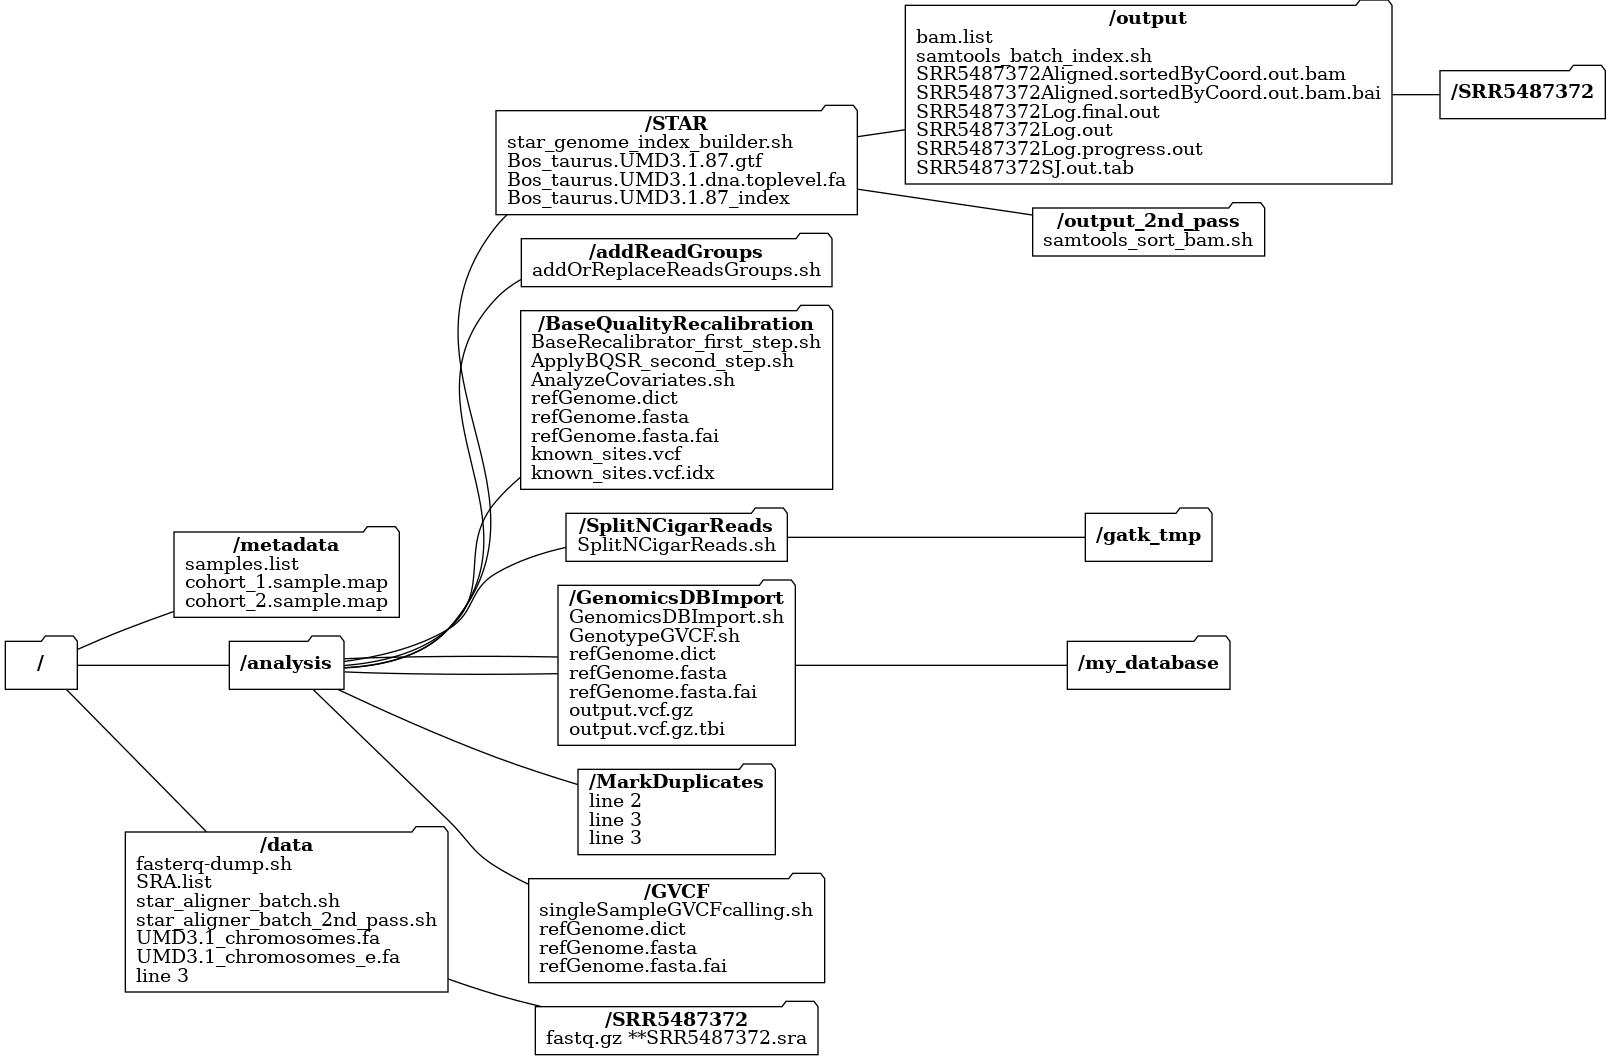
\includegraphics[width=\textwidth]{misc/tree.png}
\caption[caption] {long desc.}

\end{center}
\end{figure}





\subsection{Downloading sequences from NCBI SRA}

In this tutorial, we choose to work with full-length RNAseq datasets derived from macrophage transcriptomes of cows in response to the infection by \textit{Mycobacterium avium ssp. paratuberculosis } (MAP), the etiological agent of paratuberculosis, or Johne’s disease (JD) \cite{Ariel2021}. A representative subset of 24 samples was selected for which the SRA identifiers can be found in the data/SRA.list file.

\begin{verbatim}
SRS2153774
SRS2153779
SRS2153781
...
SRS2153841
SRS2153845
\end{verbatim}


To download these sequences (221 Gb), navigate to the /data directory and download the samples with the prefetch command from the SRAtoolkit:

\begin{verbatim}
prefetch --option-file SRA.list
\end{verbatim}

To extract fastq files from .sra archives, the fasterq-dump command is required. For example, the following command will produce SRR5487396\_R1.fastq.gz and SRR5487396\_R2.fastq.gz:

\begin{verbatim}
fasterq-dump --split-files SRR5487396/SRR5487396.sra
\end{verbatim}

In practice, you will want to extract all downloaded sequence read archives, which are nested in distinct folders. Navigate to the /data folder and use the following qsub command to lauch the faster-qdump commands sequentially:

\begin{verbatim}
qsub -V -S /bin/bash -cwd -j y -pe smp 12 faster-qdump_sequential.sh
\end{verbatim}

where faster-qdump\_sequential.sh is a BASH script containing instructions for the SGE workload manager as well as the code to iterate on the downloaded archives and to produce the forward and reverse fastq files:

\begin{verbatim}
#! /bin/bash
#$ -N 'fasterq-dump'
#$ -o ./faster-qdump_log.txt
for i in `ls -d SRR*`; do
	cd $i; fasterq-dump --split-files $i.sra; cd ..
done
\end{verbatim}


However, executing the latter script would take a lot of times. To take advantage of the parallel computing capacity of compute servers, one may consider launching SGE task array jobs (tasks in parallel). This can be done by using the SGE task array capabilities. Briefly, a single script is run multiple times with different values taken by the single environment variable \$SGE\_TASK\_ID. Using an UNIX trick on a list of samples, each instance of the script can be run on a distinct dataset. Since many bioinformatic tasks used in this tutorial are computationally intensive, most of the scripts presented thereafter will be base on this model. For brevity, we did not include most of the required SGE options (lines beginning with \#\$ within BASH scripts. Therefore, it is important to include them in the qsub command. In this tutorial, all parallel tasks (with 24 samples) should be launched with command such as:
\begin{verbatim}
qsub -V -S /bin/bash -cwd -j y -t 1-24 -pe smp 4 parallel_task.sh \
\end{verbatim}

Otherwise, omit the -t option and increase the number of cores to be used:
\begin{verbatim}
qsub -V -S /bin/bash -cwd -j y -pe smp 12 unparallel_task.sh \
\end{verbatim}

Before lauching the parallel version of fasterq.dump.sh, create a simple list of the 24 SRR* folders present in the /data folder:

\begin{verbatim}
ls -d1 SRR5487???>SRR.list
\end{verbatim}

The SRR.list file should contain the 24 SRR identifiers (without the .sra extension) on separates lines. You are now ready to execute the faster-qdump\_parallel.sh listing:

\begin{verbatim}
#!/bin/bash
#$ -N fasterq-dump
#$ -o ./fasterq-dump.$TASK_ID.log
input=$(head -n $SGE_TASK_ID SRR.list | tail -n 1)
cd $input
fasterq-dump --split-files $input.sra
cd ..
\end{verbatim}












